\documentclass{article}
\usepackage{v-test-paper}
\usepackage{mathtools}
\usepackage{tikz-3dplot}
\usepackage[pages=some]{background}


\backgroundsetup{
  scale=1,
  color=black!90,
  opacity=1,
  angle=0,
  position=current page.south west,
  vshift=0,
  hshift=0,
  contents={
    \begin{tikzpicture}[remember picture, overlay]
      \fill[pattern=dots, pattern color=black!35] (current page.south west) rectangle (current page.north east);
    \end{tikzpicture}
  },
}

\newenvironment{solution}{\par\noindent\color{red!85!black}$\Rightarrow$\vspace{0em}}{}

\ExplSyntaxOn
\NewDocumentCommand{\vbsubtitle}{O{} m}
{
  \textscale{#1}{#2}
}

\NewDocumentCommand{\textscale}{ m m}
{
  \tl_if_empty:nTF {#1}
  {
    \textsc{#2}
  }
  {
    \scalebox{#1}{\textsc{#2}}
  }
}


\NewDocumentCommand{\vbdefinition}{m}
{
  \begin{quote}
  \textit{#1}
  \end{quote}
}


\NewDocumentCommand{\vbtitle}{O{\large} m}
{
  \begin{center}
    #1 \textsc{#2}
  \end{center}
}

\ExplSyntaxOff



\title{\textsc{Coordinate System}}

\begin{document}
\maketitle


    \begin{itemize}
    \item Location of a point on a line
    \begin{quote}
        \textit{
            Imagine a world where you can only move in two directions: forward and backward. You can't move left or right, up or down—only along a single straight path. This path is called the x-axis. The x-axis is a horizontal line that extends infinitely in both directions. \\[2mm]
            In this one-dimensional world, we can describe the location of any point using a single number, which we call the coordinate of that point. This number tells us exactly how far along the x-axis the point is from a specific reference point known as the origin. The origin is the center point of the x-axis and has a coordinate of $0$.\\[2mm]
            If a point has a positive coordinate, it means the point is to the right of the origin. If a point has a negative coordinate, it means the point is to the left of the origin. The greater the number, the further the point is from the origin.
        }
    \end{quote}

        \begin{center}
            \begin{tikzpicture}
                \tzaxes(-5, 0)(5, 0.15){$x$}{}
                \tzticks{-4/$-4$, -3/$-3$, -2/$-2$, -1/$-1$, 0/$0$, 1/$1$, 2/$2$, 3/$3$, 4/$4$}{}
                \tzticks*{-4, -3, -2, -1, 1, 2, 3, 4}{}
            \end{tikzpicture}
            \begin{tikzpicture}
                \tzaxes(-5, 0)(5, 0.15){$x$}{}
                \tzticks{-2.5/$x_1$, 2.5/$x_2$}{}
                \tzticks*{-2.5, 0, 2.5}{}
                \tzline[|<->|]<0, -0.75>(-2.5, 0)(2.5, 0){$x_2 - x_1$}[mb]
            \end{tikzpicture}
        \end{center}

    \item Location of a point in a plane
    \begin{quote}
        \textit{
            Now, imagine a world where you can move not just forward and backward, but also left and right. This world is two-dimensional, meaning it has two directions or axes along which you can move: the x-axis and the y-axis.\\[2mm]
            The x-axis is a horizontal line that runs from left to right, and the y-axis is a vertical line that runs from bottom to top. These two lines intersect at a point called the origin, which has the coordinates (0, 0).
            In this two-dimensional world, we can describe the location of any point using a pair of numbers called coordinates. These coordinates are written as (x, y):\\[2mm]
            The first number, x, tells us how far along the x-axis the point is from the origin. A positive x value means the point is to the right of the origin, while a negative x value means the point is to the left.
            The second number, y, tells us how far along the y-axis the point is from the origin. A positive y value means the point is above the origin, while a negative y value means the point is below.
        }
    \end{quote}

        \begin{center}
            \begin{tikzpicture}
                \tzaxes(-5, -3)(5, 4){$x$}{$y$}
                \tzticks*{-4, -3, -2, -1, 1, 2, 3, 4}{-2, -1, 1, 2, 3}
                \tzcoor*(0, 0)(O){$O$}[bl]
                \tzcoor*(2, 3)(P){$P(2,3)$}[ar]
                \tzline[|<->|]<0, -0.5>(0, 0)(2, 0){$2$}[mb]
                \tzline[|<->|]<2.5, 0>(0, 0)(0, 3){$3$}[mr]
            \end{tikzpicture}
        \end{center}

        \textbf{Coordinates of a point $P(x, y)$:} \\
        
        \begin{itemize}
            \item \textbf{Distance between two points:}
                \begin{center}
                    \begin{tikzpicture}
                        \tzaxes(-2, -1.5)(7, 4){$x$}{$y$}
                        \tzcoor*(0, 0)(O){$O$}[bl]
                        \tzcoor*(2, 3)(P){$P(x_1, y_1)$}[ar]
                        \tzcoor*(5, 1)(Q){$Q(x_2, y_2)$}[ar]
                        \tzline[dashed](2, 1)(5, 1){$x_2-x_1$}[mb]
                        \tzline[dashed](2, 1)(2, 3){$y_1-y_2$}[ml]
                        \tzline(P)(Q){$d$}[ma]
                        \tzline[|<->|]<0, -0.5>(0, 0)(2, 0){$x_1$}[mb]
                        \tzline[|<->|]<0, -1>(0, 0)(5, 0){$x_2$}[mb]
                        \tzline[|<->|]<-0.5, 0>(0, 0)(0, 1){$y_2$}[ml]
                        \tzline[|<->|]<-1, 0>(0, 0)(0, 3){$y_1$}[ml]
                    \end{tikzpicture}
                \end{center}
                \begin{align*}
                    \intertext{Distance between two points $P(x_1, y_1)$ and $Q(x_2, y_2)$:}
                    \intertext{Using Pythagoras theorem:}
                    \Aboxed{d &= \sqrt{(x_2 - x_1)^2 + (y_2 - y_1)^2}}
                \end{align*}

            \item \textbf{Midpoint of a line segment:}
                \begin{center}
                    \begin{tikzpicture}
                        \tzcoor*(2, 3)(P){$P(x_1, y_1)$}[ar]
                        \tzcoor*(5, 1)(Q){$Q(x_2, y_2)$}[ar]
                        \tzcoor*(3.5, 2)(M){$M(x_m, y_m)$}[ar]
                        \tzline[dashed](2, 1)(5, 1){$x_2-x_1$}[mb]
                        \tzline[dashed](2, 1)(2, 3){$y_1-y_2$}[ml]
                        \tzline(P)(Q)
                        \tzline[dashed](2, 2)(M){$x_m-x_1$}[mb]
                        \tzline[dashed, |<->|]<-1.5, 0>(2, 2)(2, 3){$y_1-y_m$}[ml]
                    \end{tikzpicture}
                \end{center}
                \begin{align*}
                    \intertext{Midpoint of a line segment $P(x_1, y_1)$ and $Q(x_2, y_2)$:}
                    \intertext{From the above diagram, we can see that both the triangles are similar.}
                    \intertext{Therefore,}
                    \frac{y_1-y_m}{y_1-y_2} &= \frac{x_m-x_1}{x_2-x_1} = \frac{PM}{PQ} \\
                    \intertext{As the midpoint divides the line segment into two equal parts,}
                    \frac{y_1-y_m}{y_1-y_2} &= \frac{x_m-x_1}{x_2-x_1} = \frac{1}{2}
                \end{align*}
                \begin{align*}
                    \intertext{Solve for $x_m$ and $y_m$:}
                    \frac{x_m - x_1}{x_2 - x_1} &= \frac{1}{2}  &\text{and}&& \frac{y_1 - y_m}{y_1 - y_2} &= \frac{1}{2} \\
                    x_m - x_1 &= \frac{x_2 - x_1}{2}  &\text{and}&& y_1 - y_m &= \frac{y_1 - y_2}{2} \\
                    x_m &= \frac{x_1 + x_2}{2}  &\text{and}&&  y_m &= \frac{y_1 + y_2}{2}
                \end{align*}
                \begin{align*}
                    \Aboxed{M(x_m, y_m) &= \left(\frac{x_1 + x_2}{2}, \frac{y_1 + y_2}{2}\right)}
                \end{align*}
        \end{itemize}

\end{itemize}

    % \vbtitle{\textbf{Illustrations: Coordinate System}}

\begin{enumerate}
    \item 
\end{enumerate}

    \begin{center}
    \textsc{\Large\textbf{Slope of a line}}
\end{center}
    \begin{center}
        \begin{tikzpicture}
            \tzaxes(-2, -1.5)(7, 4){$x$}{$y$}
            \tzline"L1"(0, 0)(6, 4){$L_1(x)$}[ar]
            \tzline"L2"(0, 0)(6, 2){$L_2(x)$}[ar]
            \tzline[dashed]"DL"(4, 0)(4, 4)
            \tzXpoint{DL}{L1}(X1)
            \tzXpoint{DL}{L2}(X2)
            \tzdot*(X1)
            \tzdot*(X2)
            \tzline[|<->|]<0, -0.5>(0, 0)(4, 0){$\Delta x$}[mb]
            \tzline[|<->|]<0.5, 0>(4, 0)(X2){$\Delta y_2$}[mr]
            \tzline[|<->|]<1.5, 0>(4, 0)(X1){$\Delta y_1$}[mr]
        \end{tikzpicture}
    \end{center}
    \begin{quote}
        \textit{
            The slope of a line is a measure of its steepness and direction, and it can be interpreted as the rate of change of the line. It is calculated as the ratio of the vertical change to the horizontal change between two distinct points on the line.\\[2mm]
            In the above diagram $L_1$ and $L_2$ are two lines, $\Delta x$ is the horizontal change, and $\Delta y_1$ and $\Delta y_2$ are the vertical changes of the lines $L_1$ and $L_2$ respectively.\\[2mm]
            As you can see $\Delta y_1 > \Delta y_2$ and $\Delta x$ is the same for both the lines. Therefore, the slope of the line $L_1$ is greater than the slope of the line $L_2$.\\[2mm]
            Here, for both the lines $L_1$ and $L_2$, for $\Delta x > 0$, $\Delta y_1 \textit{ and } \Delta y_2$ are positive. Therefore, the slope of the line is positive.
        }
    \end{quote}
    \begin{itemize}
        \item But slope can be negative if $\Delta y < 0$ for $\Delta x > 0$.
            \begin{center}
                \begin{tikzpicture}
                    \tzaxes(-2, -1)(7, 4){$x$}{$y$}
                    \tzcoors*(1,1)(A)(1,2)(B)(3,1)(C);
                    \tzLFn(B)(C)[-1:5]
                    \tzline[dashed](A)(B)
                    \tzline[dashed](A)(C)
                    \tzline[|<->|]<-0.25, 0>(A)(B){$\Delta y$}[ml]
                    \tzline[|<->|]<0, -0.25>(A)(C){$\Delta x$}[mb]
                \end{tikzpicture}
            \end{center}

        \item Slope can be zero if $\Delta y = 0$ for all $\Delta x \neq 0$.
            \begin{center}
                \begin{tikzpicture}
                    \tzaxes(-2, -1)(7, 3.5){$x$}{$y$}
                    \tzcoors*(1, 2)(A)(3, 2)(B);
                    \tzLFn(A)(B)[-1:5]
                    \tzline[|<->|]<0, -0.25>(A)(B){$\Delta x$}[mb]
                \end{tikzpicture}
            \end{center}

        \item Slope can be undefined if $\Delta x = 0$\\
            In this case, the line is vertical, meaning the slope tends to infinity. This situation violates the definition of slope because the slope is the ratio of the vertical change to the horizontal change. However, when the horizontal change is zero but the vertical change is not zero, this ratio becomes undefined.
            \begin{center}
                \begin{tikzpicture}
                    \tzaxes(-2, -1)(7, 4){$x$}{$y$}
                    \tzcoors*(1, 1)(A)(1, 3)(B);
                    % \tzLFn(A)(B)[-1:5]
                    \tzline($(A)+(0, -1.5)$)($(B)+(0, 1)$)
                    \tzline[|<->|]<-0.25, 0>(A)(B){$\Delta y$}[ml]
                \end{tikzpicture}
            \end{center}
    \end{itemize}
    % \pagebreak
\vspace*{10mm}
    \begin{center}
        \textsc{Slope of a line passing through two points $P(x_1, y_1)$ and $Q(x_2, y_2)$}\\[10mm]
        \begin{tikzpicture}
            \tzaxes(-2, -1)(7, 4){$x$}{$y$}
            \tzcoors*(4,1)(A)(1,1)(B){$P(x_1, y_1)$}[al](4,3)(C){$Q(x_2, y_2)$}[al];
            \tzLFn(B)(C)[-1:5]
            \tzline[dashed](A)(B)
            \tzline[dashed](A)(C)
            \tzline[|<->|]<0, -0.5>(A)(B){$\Delta x$}[mb]
            \tzline[|<->|]<0.5, 0>(A)(C){$\Delta y$}[mr]
            \tzanglemark(A)(B)(C){$\theta$}(15pt)
        \end{tikzpicture}
    \end{center}
    \begin{align*}
        \intertext{Slope of a line passing through two points $P(x_1, y_1)$ and $Q(x_2, y_2)$:}
        \textit{Slope(m) } &= \frac{\Delta y}{\Delta x} \\
        \intertext{From the above diagram,}
        \tan \theta &= \frac{\Delta y}{\Delta x} \\
        \intertext{Therefore,}
        \Aboxed{m &= \tan \theta = \frac{y_2 - y_1}{x_2 - x_1}}
        \intertext{Be careful, $\theta$ is the angle between the line and the positive x-axis in anti-clockwise direction.}
    \end{align*}
    \begin{center}
    \textsc{\Large\textbf{Locus of a Point}}
\end{center}

\begin{center}
    \begin{tikzpicture}
        \tzcoor*(0, 0)(O)
        \foreach \A in {0, 20,..., 340}{
            \tzdot*(\A:2)
            \tzline[dashed](O)(\A:2)
            \tzline[->](\A:2)(\A + 10:2)
        }
    \end{tikzpicture}
\end{center}


\begin{quote}
    Imagine you're at a park with a beautiful fountain at the center. You and your friend decide to play a game where you always stay exactly 10 feet away from the fountain.

    You start walking, keeping that distance constant. As you move around the fountain, you notice your feet are tracing a perfect circle with the fountain at the center. This path your feet are creating is called the \textbf{locus}.

    In geometry, a locus is the set of all points that satisfy a specific condition. In this game, the locus is the circle formed by your feet always being 10 feet from the fountain.

    So, the locus is just a fancy way of describing the path or shape created by a point (in this case, your feet) moving according to certain rules.
\end{quote}

\begin{quote}
    \textit{
        A locus is essentially the path traced out by a moving point that moves according to a specific set of conditions or rules.
    }
\end{quote}

\vspace*{10mm}

\begin{center}
    \textsc{\large Equation of a Line}
\end{center}

\begin{quote}
    \textit{
        A line can be defined as the locus of a point that moves in such a way that it maintains a constant rate of change between its coordinates. This constant rate of change is known as the slope. \\[2mm]
    }
\end{quote}

\begin{center}
    \begin{tikzpicture}
        \tzcoor*(2, 2)(P){$P(x_1, y_1)$}[al]
        \tzcoor*(5, 4)(Q){$Q(x_2, y_2)$}[al]
        \tzcoor*($0.5*(P) + 0.5*(Q)$)(M){$M(x, y)$}[al]
        \tzLFn(P)(Q)[1:6]
    \end{tikzpicture}
\end{center}

\begin{quote}
    Consider two fixed points \( P(x_1, y_1) \) and \( Q(x_2, y_2) \) and a moving point \( M(x, y) \). This moving point will change its location such that it maintains a constant slope from any point on the line.
\end{quote}

\begin{align*}
    \intertext{As these two points $P$ and $Q$ lie on the line,}
    \textit{Slope of PM } &= \textit{ Slope of MQ} \\
    \frac{y - y_1}{x - x_1} &= \frac{y_2 - y}{x_2 - x} \\
    (y-y_1)(x_2-x) &= (y_2-y)(x-x_1) \\
    yx_2 - yx - y_1x_2 + y_1x &= y_2x - y_2x_1 - yx + yx_1 \\
    x\left(y_1-y_2\right) + y\left(x_2-x_1\right) + x_1y_2 - x_2y_1 &= 0 \\
    \intertext{Now, we can replace the constants with \( a = y_1 - y_2 \), \( b = x_2 - x_1 \), \( c = x_1y_2 - x_2y_1 \)}
    \Aboxed{ax + by + c &= 0}
\end{align*}

\begin{itemize}
    \item \textbf{Point-slope form:}\\[2mm]
    Let's consider a fixed point \( P(x_1, y_1) \) and a moving point \( M(x, y) \) on a line with a given slope \( m \). We are interested in finding the equation of the line that passes through the point \( P(x_1, y_1) \) and has a slope \( m \).\\[2mm]
        \begin{center}
            \begin{tikzpicture}
                \tzaxes(-2, -1)(7, 4){$x$}{$y$}
                \tzcoor*(2, 2)(P){$P(x_1, y_1)$}[al]
                \tzcoor*(4, 3)(M){$M(x, y)$}[al]
                \tzLFn(P)(M)[0.5:5]
            \end{tikzpicture}
        \end{center}
        \begin{align*}
            \intertext{According to the definition of slope,}
            \textit{Slope(m) } &= \frac{y - y_1}{x - x_1} \\
            \intertext{Therefore,}
            \Aboxed{y - y_1 &= m(x - x_1)}
        \end{align*}

    \item \textbf{Slope and intercept(y) form:}\\[2mm]
    Let's consider a line with slope \( m \) and y-intercept \( c \). We are interested in finding the equation of the line that has a slope \( m \) and y-intercept \( c \).\\[2mm]
        \begin{center}
            \begin{tikzpicture}
                \tzaxes(-2, -1)(6, 4){$x$}{$y$}
                \tzcoor*(0, 1)(P){$P(0, c)$}[al]
                \tzcoor*(4, 3)(M){$M(x, y)$}[al]
                \tzLFn(P)(M)[-1:5]
            \end{tikzpicture}
        \end{center}
        \begin{align*}
            \intertext{According to the definition of slope,}
            \textit{Slope(m) } &= \frac{y - c}{x - 0} \\
            \intertext{Therefore,}
            \Aboxed{y &= mx + c}
        \end{align*}

    \pagebreak
    \item \textbf{Two-point form:}\\[2mm]
    Let's consider two fixed points \( P(x_1, y_1) \) and \( Q(x_2, y_2) \) on a line. We are interested in finding the equation of the line that passes through the points \( P(x_1, y_1) \) and \( Q(x_2, y_2) \).\\[2mm]
        \begin{center}
            \begin{tikzpicture}
                \tzaxes(-2, -1)(7, 4){$x$}{$y$}
                \tzcoor*(2, 2)(P){$P(x_1, y_1)$}[al]
                \tzcoor*(5, 3.5)(Q){$Q(x_2, y_2)$}[al]
                \tzcoor*($0.5*(P) + 0.5*(Q)$)(M){$M(x, y)$}[al]
                \tzLFn(P)(Q)[1:6]
            \end{tikzpicture}
        \end{center}
        \begin{align*}
            \intertext{According to the definition of line,}
            \textit{Slope of PQ } &= \textit{ Slope of PM} \\
            \frac{y_2 - y_1}{x_2 - x_1} &= \frac{y - y_1}{x - x_1} \\
            \intertext{Therefore,}
            \Aboxed{y - y_1 &= \frac{y_2 - y_1}{x_2 - x_1}(x - x_1)}
        \end{align*}

    \item \textbf{Intercept form:}\\[2mm]
    Let's consider a line with x-intercept \( a \) and y-intercept \( b \). We are interested in finding the equation of the line that has x-intercept \( a \) and y-intercept \( b \).\\[2mm]
        \begin{center}
            \begin{tikzpicture}
                \tzaxes(-2, -2)(6, 3.5){$x$}{$y$}
                \tzcoor*(3, 0)(P){$P(a, 0)$}[bl]
                \tzcoor*(0, 2)(Q){$Q(0, b)$}[ar]
                \tzcoor*($0.5*(P) + 0.5*(Q)$)(M){$M(x, y)$}[ar]
                \tzLFn(P)(Q)[-1:5]
            \end{tikzpicture}
        \end{center}
        \begin{align*}
            \intertext{According to the definition of line,}
            \textit{Slope of PQ
            } &= \textit{ Slope of PM} \\
            \frac{b - 0}{0 - a} &= \frac{y - 0}{x - a} \\
            b\left(x-a\right) &= -ay \\
            \intertext{Divide both sides by \( ab \),}
            \Aboxed{\frac{x}{a} + \frac{y}{b} &= 1}
        \end{align*}

\end{itemize}
    \begin{center}
    \textsc{\large\textbf{Illustrations: Slope, Line}}
\end{center}
\BgThispage
\begin{enumerate}
    \item Find the slope and also write the equation of the given straight lines:
        \begin{tasks}(2)
            \task 
                \begin{center}
                    \begin{tikzpicture}[scale=0.75]
                        \tzaxes(-1, -2)(4, 2){$x$}{$y$}
                        \tzcoors*(2, 1)(B){$(2,1)$}[al](0, -1)(A){$(0, -1)$}[l];
                        \tzLFn(A)(B)[-1:2.5]
                    \end{tikzpicture}
                \end{center}

            \task
                \begin{center}
                    \begin{tikzpicture}[scale=0.75]
                        \tzaxes(-1, -1)(4, 3){$x$}{$y$}
                        \tzcoors*(0, 2)(A)(2, 0)(B){$2$}[bl];
                        \tzLFn(A)(B)[-1:3]
                        \tzanglemark(3, 0)(B)(A){$135^\circ$}[pos=2.5]
                    \end{tikzpicture}
                \end{center}

            \task 
            \begin{center}
                \begin{tikzpicture}[scale=0.75]
                    \tzaxes(-1, -1.5)(4, 3){$x$}{$y$}
                    \tzcoors*(0, 2)(A)(1.5, 0)(B){$1$}[bl];
                    \tzLFn(A)(B)[-0.8:2.75]
                    \tzanglemark'(B)(A)(0, 3){$150^\circ$}[pos=2.5]
                \end{tikzpicture}
            \end{center}

            \task 
                \begin{center}
                    \begin{tikzpicture}[scale=0.75]
                        \tzaxes(-1, -1)(4, 3){$x$}{$y$}
                        \tzcoors*(0, 0)(A)(2.5, 1.5)(B){$(3, \sqrt{3})$}[al];
                        \tzLFn(A)(B)[-1:3]
                    \end{tikzpicture}
                \end{center}
            
            \task 
                \begin{center}
                    \begin{tikzpicture}[scale=0.75]
                        \tzaxes(-3, -1)(3, 3){$x$}{$y$}
                        \tzcoors*(-2, 0)(A){$-2$}[b](0, 1)(B){$1$}[al];
                        \tzLFn(A)(B)[-3:2.5]
                    \end{tikzpicture}
                \end{center}

            \task
                \begin{center}
                    \begin{tikzpicture}[scale=0.75]
                        \tzaxes(-1, -1)(4, 3){$x$}{$y$}
                        \tzcoors*(0, 2)(A){$2$}[al](2, 2)(B){$(2, 2)$}[ar];
                        \tzLFn(A)(B)[-1:3]
                        \tzline[dashed] (2, 0)(2, 3)
                    \end{tikzpicture}
                \end{center}

            \task
                \begin{center}
                    \begin{tikzpicture}[scale=0.75]
                        \tzaxes(-1, -1)(4, 3){$x$}{$y$}
                        \tzcoors*(2, 0)(B){$2$}[br];
                        \tzline(2, -1)(2, 2.5)
                        \tzrectangle(2, 0)(2.4, 0.4)
                    \end{tikzpicture}
                \end{center}

            \task
                \begin{center}
                    \begin{tikzpicture}[scale=0.75]
                        \tzaxes(-1, -1)(4, 3){$x$}{$y$}
                        \tzcoors*(0, 0)(A);
                        \tzline(0, 0)(3, 3)
                        \tzanglemark(3, 0)(0, 0)(3, 3){$45^\circ$}[pos=2.5]
                    \end{tikzpicture}
                \end{center}
        \end{tasks}
        
        \begin{solution}
           
            \begin{enumerate}
                \item 
                    \begin{align*}
                        \intertext{We can use the two-point form to find the slope of the line. Slope:}
                        m &= \frac{y_2-y_1}{x_2-x_1} = \frac{1-(-1)}{2-0} = 1
                        \intertext{For the equation of the line, we can use the slope-intercept form. Equation:}
                        y &= mx + c \\
                        y &= x - 1
                    \end{align*}

                \item
                    \begin{align*}
                        \intertext{We can use $\tan\theta$ as the $\theta$ is known here. Slope:}
                        m &= \tan 135^\circ = \tan (180^\circ - 45^\circ) = -\tan 45^\circ = -1
                        \intertext{For the equation of the line, we can use the slope-point form. Equation:}
                        y - y_1 &= m(x - x_1) \\
                        y - 0 &= -1(x - 2) \\
                        y &= -x + 2
                    \end{align*}

                \item
                \begin{multicols}{2}
                    \begin{align*}
                        \intertext{We can use $\tan\theta$ as the $\theta$ is known here. Slope:}
                        m &= \tan 120^\circ \\
                        &= \tan (180^\circ - 60^\circ) \\
                        &= -\tan 60^\circ \\
                        &= -\sqrt{3}
                        \intertext{For the equation of the line, we can use the slope-point form. Equation:}
                        y - y_1 &= m(x - x_1) \\
                        y - 0 &= -\sqrt{3}(x - 1) \\
                        y &= -\sqrt{3}x + \sqrt{3}
                    \end{align*}
                    \begin{center}
                        \begin{tikzpicture}[scale=0.75]
                            \tzaxes(-1, -1.5)(4, 4){$x$}{$y$}
                            \tzcoors*(0, 2)(A)(1.5, 0)(B){$1$}[bl];
                            \tzLFn(A)(B)[-0.8:2.75]
                            \tzanglemark'(B)(A)(0, 3){$150^\circ$}[pos=2.5]
                            \tzanglemark(0, 0)(A)(B){$30^\circ$}[pos=2](15pt)
                            \tzanglemark(A)(B)(0, 0){$60^\circ$}[pos=2]
                            \tzanglemark(4, 0)(B)(A){$120^\circ$}[pos=2](12pt)
                        \end{tikzpicture}
                    \end{center}
                \end{multicols}
                \BgThispage
                \item
                    \begin{align*}
                        \intertext{We can use the two-point form to find the slope of the line. Slope:}
                        m &= \frac{y_2-y_1}{x_2-x_1} = \frac{\sqrt{3}-0}{3-0} = \frac{1}{\sqrt{3}}
                        \intertext{For the equation of the line, we can use the slope-intercept form. Equation:}
                        y &= mx + c \\
                        y &= \frac{1}{\sqrt{3}}x
                    \end{align*}

                \item
                    \begin{align*}
                        \intertext{We can use $\tan\theta$ in the triangle formed by line and both axes. Slope:}
                        m &= \tan \theta = \frac{1}{2}
                        \intertext{For the equation of the line, we can use the slope-intercept form. Equation:}
                        y &= mx + c \\
                        y &= \frac{1}{2}x + 1
                    \end{align*}

                \item
                    \begin{align*}
                        \intertext{Line is horizontal, slope is zero.}
                        m &= 0
                        \intertext{For the equation of the line, we can use the slope-intercept form. Equation:}
                        y &= mx + c \\
                        y &= 2
                    \end{align*}

                \item
                    \begin{align*}
                        \intertext{Line is vertical, slope is undefined.}
                        m &= \text{undefined}
                        \intertext{For the equation of the line, we can observe that for every value of $y$, $x$ remains $2$. Equation:}
                        x &= 2\\[5mm]
                        \intertext{or, we can use the intercept form. Equation:}
                        \frac{x}{a} + \frac{y}{b} &= 1 \\
                        \intertext{$a=2$, $b \to \infty/-\infty$}
                        \frac{x}{2} &= 1\\
                        x &= 2
                    \end{align*}

                \item
                    \begin{align*}
                        \intertext{We can use $\tan\theta$. Slope:}
                        m &= \tan \theta = \tan 45^\circ = 1
                        \intertext{For the equation of the line, we can use the slope-intercept form. Equation:}
                        y &= mx + c \\
                        y &= x
                    \end{align*}
            \end{enumerate}
            \BgThispage
        \end{solution}

    \item Find the point of intersection of lines $y=x+4 \quad \text{and} \quad y=2x$. Also, find the equation of the line passing through their point of intersection and having slope $-1$.
        \begin{solution}
            \begin{align*}
                y &= x + 4 \\
                y &= 2x \\
                \intertext{Equating the two equations,}
                x + 4 &= 2x \\
                x &= 4 \\
                \intertext{Substituting the value of $x$ in the second equation,}
                y &= 2(4) = 8 \\
                \intertext{The point of intersection is $(4, 8)$.}
                \intertext{The equation of the line passing through the point of intersection and having slope $-1$ is}
                y - y_1 &= m(x - x_1) \\
                y - 8 &= -1(x - 4) \\
                y - 8 &= -x + 4 \\
                y &= -x + 12
            \end{align*}
        \end{solution}

    
    \item Find the angle between the straight lines $x-y=0$ and $x+y=0$.
        \begin{solution}
            \begin{align*}
                x - y &= 0 \\
                y &= x \\
                m_1 &= 1 \tag{1}\\
                x + y &= 0 \\
                y &= -x \\
                m_2 &= -1 \tag{2}
                \intertext{The angle between two lines is given by}
                \tan \theta &= \left| \frac{m_2 - m_1}{1 + m_1m_2} \right| \\
                \tan \theta &= \left| \frac{-1 - 1}{1 + 1(-1)} \right| \\
                \tan \theta &= \left| \frac{-2}{0} \right| \\
                \tan \theta &\to \infty \\
                \theta &= 90^\circ
            \end{align*}        
        \end{solution}
        \BgThispage
    \item Find the equation of the straight line passing through $(2, 3)$ and perpendicular to the straight line passing through $(-1, 0)$ and (3, 8).
        \begin{solution}
            \begin{align*}
                \intertext{The slope of the line passing through $(-1, 0)$ and $(3, 8)$ is}
                m &= \frac{8-0}{3-(-1)} = \frac{8}{4} = 2
                \intertext{The slope of the line perpendicular to this line is}
                m &= -\frac{1}{2}
                \intertext{The equation of the line passing through $(2, 3)$ and having slope $-\frac{1}{2}$ is}
                y - y_1 &= m(x - x_1) \\
                y - 3 &= -\frac{1}{2}(x - 2) \\
                y - 3 &= -\frac{1}{2}x + 1 \\
                y &= -\frac{1}{2}x + 4
            \end{align*}
        \end{solution}
\end{enumerate}



    \vbtitle{Equation of a Circle}

\vbdefinition{A circle can be defined as the locus of a point that moves in such a way that it maintains a constant distance from a fixed point. This fixed point is known as the center of the circle, and the constant distance is known as the radius.}

\begin{center}
    \begin{tikzpicture}
        \tzline[->](-3, -1)(4, -1){$x$}[r]
        \tzline[->](-1, -3)(-1, 3.5){$y$}[a]
        \tzcoor*(0, 0)(O){$O(x_0, y_0)$}[l]
        \tzcircle[dashed](O)(2)
        \tzcoor*(30:2)(M){$M(x, y)$}[r]
        \tzline+[->](M)(120:1)
        \tzline[dashed](O)(M){$r$}[mb]
    \end{tikzpicture}
\end{center}

\begin{align*}
    \intertext{Consider a fixed point $O(x_0, y_0)$ and a moving point $M(x, y)$ such that the distance between $O$ and $M$ is constant.}
    OM &= r \\
    \sqrt{(x - x_0)^2 + (y - y_0)^2} &= r \\
    \Aboxed{(x - x_0)^2 + (y - y_0)^2 &= r^2}\\[5mm]
\end{align*}

\begin{center}
    \begin{tikzpicture}
        \tzaxes(-3, -3)(3, 3){$x$}{$y$}
        \tzcoor*(0, 0)(O){$O$}[bl]
        \tzcircle[dashed](O)(2)
        \tzcoor*(30:2)(M){$M(x, y)$}[r]
        % \tzline+[->](M)(120:1)
        \tzline[->](O)(M){$r$}[mb]
    \end{tikzpicture}
\end{center}

\begin{align*}
    \intertext{If center of the circle is at the origin, $O(0, 0)$, then the equation of the circle becomes}
    \Aboxed{x^2 + y^2 &= r^2}\\[5mm]
\end{align*}

    \vbtitle{\textbf{Illustrations: Circle}}
\BgThispage
\begin{enumerate}
    \item Find the center and radius of the circle with the equation \( x^2 + y^2 - 4x - 6y - 12 = 0 \).
    \begin{solution}
        \begin{align*}
            x^2 + y^2 - 4x - 6y - 12 &= 0 \\
            x^2 - 4x + y^2 - 6y &= 12 \\
            x^2 - 4x + 4 + y^2 - 6y + 9 &= 12 + 4 + 9 \\
            (x - 2)^2 + (y - 3)^2 &= 25
        \end{align*}
        The center of the circle is \( (2, 3) \) and the radius is \( 5 \).
    \end{solution}

    \item Two straight lines \( 3x + 4y - 3 = 0 \) and \( 4x - 3y - 4 = 0 \) intersect at the point \( A \). Find the equation of the circle with \( A \) as the center and \( 5 \) as the radius.
    \begin{solution}
        \begin{align*}
            3x + 4y - 3 &= 0 \\
            4x - 3y - 4 &= 0 \\
            \intertext{Multiplying the first equation by 3 and the second equation by 4, we get}
            9x + 12y - 9 &= 0 \\
            16x - 12y - 16 &= 0 \\
            \intertext{Adding the two equations, we get}
            25x - 25 &= 0 \\
            x &= 1 \\
            \intertext{Substituting the value of \( x \) in the first equation, we get}
            3 + 4y &= 3 \\
            4y &= 0 \\
            y &= 0
        \end{align*}
        The point of intersection of the two lines is \( A(1, 0) \). The equation of the circle is
        \begin{align*}
            (x - 1)^2 + (y - 0)^2 &= 5^2 \\
            (x - 1)^2 + y^2 &= 25 \\
            x^2 - 2x + 1 + y^2 &= 25 \\
            \Aboxed{x^2 + y^2 - 2x - 24 &= 0}
        \end{align*}
    \end{solution}
\end{enumerate}

\end{document}